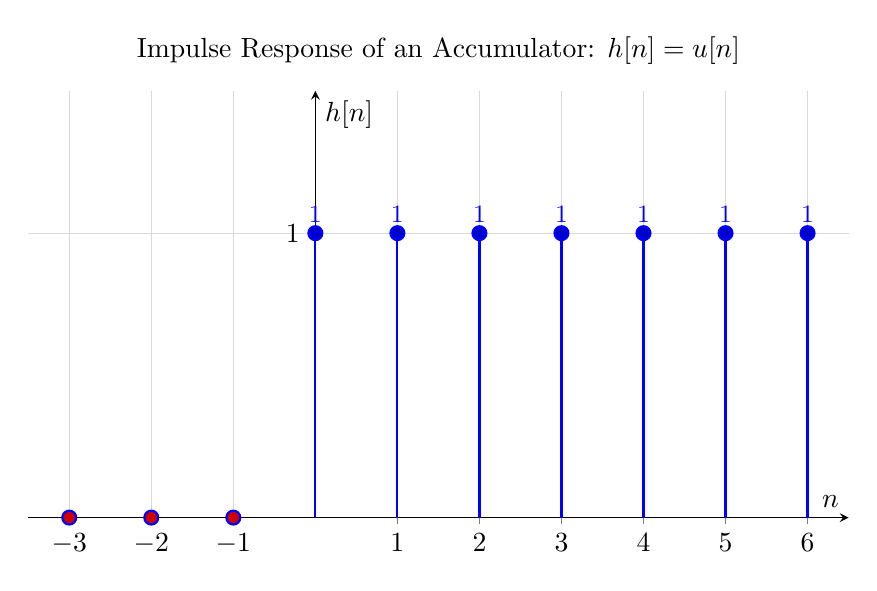
\begin{tikzpicture}
	% Define a style for our stem plots to avoid repetition
	\pgfplotsset{
		impulse/.style={
			ycomb,          % Use the 'ycomb' style for stems
			blue,           % Color of the stems and markers
			thick,          % Thickness of the stems
			mark=*,          % Marker style at the tip of the stem
			mark size=2.5pt,  % Size of the marker
		}
	}
	
	\begin{axis}[
		% Set the overall style
		width=12cm,
		height=7cm,
		% Title with context
		title={Impulse Response of an Accumulator: $h[n] = u[n]$},
		% Axis labels
		xlabel={$n$},
		ylabel={$h[n]$},
		% Position axes at the origin
		axis lines=middle,
		% Set axis limits
		xmin=-3.5, xmax=6.5,
		ymin=0, ymax=1.5,
		% Set ticks at key points
		xtick={-3, -2, -1, 0, 1, 2, 3, 4, 5, 6},
		ytick={1},
		% Add a grid
		grid=major,
		grid style={line width=.1pt, draw=gray!30},
		]
		
		% Plot the non-zero impulses and add labels above them
		\addplot+[
		impulse,
		nodes near coords={1}, % Add a '1' label to each point
		every node near coord/.style={anchor=south, font=\small}, % Position labels above
		] coordinates {
			(0, 1) (1, 1) (2, 1) (3, 1) (4, 1) (5, 1) (6, 1)
		};
		
		% Plot some zero-value points to show the effect of u[n]
		\addplot+[impulse] coordinates {
			(-3, 0)
			(-2, 0)
			(-1, 0)
		};
		
	\end{axis}
\end{tikzpicture}